% \input{"//iab.baintern.de/Dfs/017/Ablagen/D01700-Info-Board/06_WMK/Corporate Design/Folienvorlagen/TeX-Folienformat.tex"}
\input{"/Users/jonathanlatner/Google Drive/My Drive/IAB/latex/TeX-Folienformat.tex"}


\documentclass[t,10pt,utfx8]{beamer}
\usepackage{booktabs}
\usepackage{setspace}
\usepackage{parskip}
\setbeamertemplate{caption}[numbered]
\newcommand{\sprache}{\englisch}
\renewcommand{\thesubsection}{\alph{subsection})}


\title[Balancing Data Utility and Privacy: Evaluating Computer Science and Statistical approaches to Synthetic Data]{Balancing Data Utility and Privacy: Evaluating Computer Science and Statistical approaches to Synthetic Data}
\subtitle{DiskAB, 19. Juni, 2023}

\author{Jonathan Latner, PhD \newline Prof. Dr. Jörg Drechsler}

\newcounter{noauthorlines}
\setcounter{noauthorlines}{2} % Wert für 2 Autoren über 2 Zeilen. Ggf. anpassen

% %%%%%%%%%%%%%%
% Ende Anpassung
% %%%%%%%%%%%%%%

% \input{"//iab.baintern.de/Dfs/017/Ablagen/D01700-Info-Board/06_WMK/Corporate Design/Folienvorlagen/TeX-Folienformatierung_CD_2019"}
\input{"/Users/jonathanlatner/Google Drive/My Drive/IAB/latex/TeX-Folienformatierung_CD_2019"}

% Modify the section in toc template to enumerate
\setbeamertemplate{section in toc}{%
    \inserttocsectionnumber.~\inserttocsection\par
}

\setbeamertemplate{subsection in toc}{%
    \setlength{\parskip}{1mm}
    \footnotesize
    \hskip2mm -- \hskip1mm\inserttocsubsection\par
    }

\titlegraphic{\includegraphics[width=2cm]{/Users/jonathanlatner/Google Drive/My Drive/IAB/latex/CD 2019/aniged.png}}

\begin{document}


\section{Background}\label{sec_intro}
\frame[plain]{\titlepage}

\begin{spacing}{1.25}

%Table of contents
\begin{frame}
\frametitle{Sections}
\vskip6mm
\setlength{\leftskip}{0.5mm}
\setlength{\parskip}{5mm}
\begin{NoHyper}
    \footnotesize
    \tableofcontents
\end{NoHyper}
\end{frame}

\frame[c]{\frametitle{}
\centering
Section \ref{sec_intro}: Background
}


\frame{\frametitle{Comparing different packages for creating synthetic data}
\vskip -3mm
\begin{itemize}
    \footnotesize
    \item Numerous packages exit
    \item Few papers really compare and contrast
    \begin{itemize}
        \footnotesize
        \item Little et al, 2021/2023
        \item They don't tune the packages
        \item They primarily rely on data with mostly categorical data
        \item In contrast, Reiter (2005) uses mostly continuous variables: income, taxes, child suport payments, social security payments, age
    \end{itemize}
    \item The papers that do compare are often written by the authors
    \begin{itemize}
        \footnotesize
        \item In these papers, their package is often the `winner'
        \item This is not necessarily wrong
        \item This is a reflection of different strengths and weaknesses
    \end{itemize}
\end{itemize}
}

\frame{\frametitle{Summary}
\vskip -3mm
\begin{itemize}
    \footnotesize
    \item Main message: Synthpop is the `winner'
    \begin{itemize}
        \footnotesize
        \item Highest utility
        \item Fastest
        \item Little tuning required 
    \end{itemize}
    \item Datasynthesizer
    \begin{itemize}
        \footnotesize
        \item Requires tuning
        \begin{itemize}
             \item Baseline assigns equal distribution to values within any variable
             \item $k$ parents that are too high returns baseline (without warning)
         \end{itemize} 
    \end{itemize}
    \item CTGAN
    \begin{itemize}
        \footnotesize
        \item Slowest
        \item Worst performing 
    \end{itemize}
\end{itemize}
}

\frame{\frametitle{Next steps}
\begin{itemize}
    \footnotesize
    \item Simulation data
    \begin{itemize}
        \footnotesize
        \item Mixed data (categorical and continuous)
        \item Correlated variables
        \item Missing values 
    \end{itemize}
    \item Different measures of utility
    \item Different packages for creating synthetic data
    \begin{itemize}
        \footnotesize
        \item Simcity
        \item 
    \end{itemize}
    \item Privacy
\end{itemize}
}

\frame{\frametitle{Questions}
\begin{itemize}
    \footnotesize
    \item Whats my story?
    \item Is there different data that would tell a different story (i.e. relational databases)
    \item When do GANs perform well?  (i.e. not socio-economic data)
\end{itemize}
}

\section{Data}\label{sec_data}
\frame[c]{\frametitle{}
\centering
Section \ref{sec_data}: Data
}

\frame{\frametitle{Data}
\begin{itemize}
    \item 2 simulated data sets
    \begin{itemize}
        \item Isolate differences between synthetic data packages and the effect of tuning hyperparameters in a `controlled' environment 
    \end{itemize}
    \item 2 real data sets
    \begin{itemize}
        \item Benchmark our results to published papers using these data
    \end{itemize}
\end{itemize}
}

\frame{\frametitle{Simulated data}
\begin{itemize}
    \item Categorical data
    \begin{itemize}
        \item 4 bivariate categorical variables (`Y', `N')
        \item 1.000 observations
    \end{itemize}
    \item Simulated continuous data
    \begin{itemize}
        \item 3 continuous variables (`income', `wealth', `age')
        \item 1.000 observations
    \end{itemize}
    \item Simulated mixed data (continuous and categorical)
    \begin{itemize}
        \item next steps (see: Conclusion)
    \end{itemize}
\end{itemize}
}

\frame{\frametitle{Real data}
\begin{itemize}
    \item UK 1991: Individual Sample of Anonymised Records (SAR) for the British Census, subsetted on the region of West Midlands
    \begin{itemize}
        \item 20\% sample ($~ 20.000$)
        \item 12 variables: 1 numerical and 11 categorical, includes missing values
        \item Used by Little et al., 2021/2023
    \end{itemize}
    \item SD 2011: Social Diagnosis 2011 - Objective and Subjective Quality of Life in Poland
    \begin{itemize}
        \item 5.000 observations
        \item 4 variables: 2 numerical (`age', `income') and 2 categorical (`edu', `sex'), includes missing values
        \item Used by Synthpop package
    \end{itemize}
\end{itemize}
}


\section{Methods}\label{sec_methods}
\frame[c]{\frametitle{}
\centering
Section \ref{sec_methods}: Methods
}

\frame{\frametitle{Methods}
\begin{itemize}
    \item Compare 3 packages for creating synthetic data sets
    \item CTGAN (Conditional Tabular Generative Adversarial Network) in Synthetic Data Vault (SDV) package  (Patki et al., 2016)
    \item Datasynthesizer (Ping et al., 2017)
    \item Synthpop (Nowak et al., 2016)
\end{itemize}
}


\frame{\frametitle{Comparison}
\vskip -5mm
\begin{table}[h]
\caption{Comparison of Data Synthesis Methods}
\label{table_comparison}
\centering
\vskip -5mm
\begin{tabular}{lccc}
\toprule
Variable/data & CTGAN (GANs) & Datasynthesizer (PrivBayes) & Synthpop (CART) \\
\midrule
Continuous variables & \checkmark & & \\
Categorical variables & & & \checkmark \\
Mixed variables & & \checkmark & \\
Privacy protection & \checkmark$^*$ & \checkmark & \\
Relational datasets & \checkmark & & \\
High dimensional datasets & & \checkmark & \\
\bottomrule
\multicolumn{4}{p{14cm}} {\footnotesize $^*$ In theory, GANs reduce disclosure risk because they do not access the original (or training) data at all, and starts off with only noise as input.  This is also why they should be superior for continuous variables.}
\end{tabular}
\end{table}

\footnotesize
{\bf JPL Note: I think this table is wrong, but it would be nice to have something like this.}
}

\frame{\frametitle{CTGAN}
\footnotesize
\begin{itemize}
    % \item \url{https://docs.sdv.dev/sdv/}
    \item SDV is a system that builds generative models of {\bf relational databases}
    \item GANs typically train two neural network (NN) models: 
    \begin{enumerate}
        \footnotesize
        \item a generative model that captures the data distribution and generates new data samples
        \item a discriminative model that aims to determine whether a sample is from the model distribution or the data distribution
    \end{enumerate}
    \item The models are trained together in an adversarial zero-sum game, such that the generator goal is to produce data samples that fool the discriminator into believing they are real and the discriminator goal is to determine which samples are real and which are fake. 
    \item Training is iterative with (ideally) both models improving over time to the point where the discriminator can no longer distinguish which data is real or fake. 
    \item Advantages
    \begin{itemize}
        \footnotesize
        \item Continuous variables: generally considered to be superior
        \item From a privacy perspective, the generative model does not access the original (or training) data at all, and starts off with only noise as input.
    \end{itemize}
\end{itemize}
}

\frame{\frametitle{Datasynthesizer}
\footnotesize
\begin{itemize}
    % \item \url{https://github.com/DataResponsibly/DataSynthesizer}
    \item Implements a version of the PrivBayes (Zhang et al., 2017) algorithm. 
    \item Learns a differentially private Bayesian Network that captures the correlation structure between attributes and then draws samples. 
    \item Advantages
    \begin{itemize}
        \footnotesize
        \item A settable parameter, $\epsilon$, controls differential privacy. 
        \item Mixed data: Well suited to data sets with both continuous and categorical data because it models the joint distribution by incorporating the number of parents a given variable has.
        \item High dimensional data 
    \end{itemize}
\end{itemize}
}

\frame{\frametitle{Synthpop}
\footnotesize
\begin{itemize}
    % \item \url{https://www.synthpop.org.uk/}
    \item Synthpop uses CART as the default method of synthesis (other options include random forests and various parametric alternatives). 
    \item Synthpop synthesises the data sequentially, one variable at a time; the first is sampled, then the following are synthesised using the previous variables as predictors. 
    \item Advantages:
    \begin{itemize}
        \footnotesize
        \item Requires little tuning and performs very quickly
        \item Superior performance on categorical data
    \end{itemize}
\end{itemize}
}


\section{Tuning}\label{sec_tuning}
\frame[c]{\frametitle{}
\centering
Section \ref{sec_tuning}: Tuning
}

\frame{\frametitle{CTGAN}
\footnotesize
\begin{enumerate}
    \item {\bf epochs} (3: 300, 600, 900): the number of iterations that the model will perform to optimize its parameters. Default is 300.  
    \item {\bf batch\_size} (2: 500, 1000): as well as the number of samples used in each step. Default is 500.  
    \item {\bf log\_frequency} (2: True, False): Whether to use log frequency of categorical levels in conditional sampling. It defaults to True. This argument affects how the model processes the frequencies of the categorical values that are used to condition the rest of the values. In some cases, changing it to False could lead to better performance.
    \item {\bf discriminator\_steps} (3: 1, 5, 10): Number of discriminator updates to do for each generator update. Default is 1.
    \item copies (3: 1, 5, 10): Number of synthetic data sets
\end{enumerate}
Total: 108 combinations of tuning parameters (576 synthetic data sets)
}

\frame{\frametitle{Datasynthesizer}
\footnotesize
\begin{enumerate}
    \item k (3: 0, 1, 2).  The maximum number of parents in Bayesian network, i.e., the maximum number of incoming edges.  Default is 0.
    \item epsilon (7: 0, 0.1, 1, 5, 10, 20, 30).  It roughly means that removing a row in the input dataset will not change the probability of getting the same output more than a multiplicative difference of exp(epsilon).  Increase epsilon value to reduce the injected noises. Set epsilon=0 to turn off differential privacy.  Default is 0.1.
    \item copies (3: 1, 5, 10): Number of synthetic data sets
\end{enumerate}
Total: 63 combinations of tuning parameters (336 synthetic data sets)
}

\frame{\frametitle{Synthpop}
\footnotesize
\begin{enumerate}
    \item complexity parameter (5: 1e-8, 1e-6, 1e-4, 0.01).  complexity parameter. Any split that does not decrease the overall lack of fit by a factor of cp is not attempted. Small values of cp will grow large trees.  Default is 0.00000001 (1e-8).
    \item minbucket (4: 5, 10, 25, 50). the minimum number of observations in any terminal $<leaf>$ node. Default is 5.  
    \item copies (3: 1, 5, 10): Number of synthetic data sets
\end{enumerate}
Total: 48 combinations of tuning parameters (256 synthetic data sets)
}

\section{Measuring utility}\label{sec_utility}
\frame[c]{\frametitle{}
\centering
Section \ref{sec_utility}: Measuring utility \\
}

\frame{\frametitle{Measuring utility}
\footnotesize

\begin{itemize}
    \item Ratio of counts (ROC)/Ratio of estimates (ROE)
    \begin{itemize}
        \item univariate
        \item bivariate
    \end{itemize}
    \item Confidence interval overlap (CIO)
    \begin{itemize}
        \item Standardized difference of the difference in estimates (Std. Diff)
        \item CIO
    \end{itemize}
    \item Propensity score (next steps?)
    \begin{itemize}
        \item pMSE - propensity mean squared error
        \item S\_pMSE - standardized ratio (pMSE)
    \end{itemize}
    \item Others?
\end{itemize}
}


\frame{\frametitle{Ratio of counts (ROC)/Ratio of estimates (ROE)}
\footnotesize

ROC only works when both datasets are the same size, which is true here, but does not have to be true by definition.

ROE is calculated by taking the ratio of the synthetic and original data estimates (e.g. totals, proportions), where the smaller of these two estimates is divided by the larger one. Thus, given two corresponding estimates, where $y^1_{orig}$ is the estimate orig from the original data and $y^1_{synth}$ is the corresponding estimate from the synthetic synth data, the ROE is calculated as:

\begin{equation}
    ROE = \frac{min(y^1_{orig},y^1_{synth})}{max(y^1_{orig},y^1_{synth})}
\end{equation}

Max = 1, min = 0, and higher is better.  If $y^1_{orig}$ = $y^1_{synth}$, then ROE = 1.  The ROE will be calculated over bivariate and univariate data.  For each categorical variable the ratio of estimates are averaged across categories to give an overall ratio of estimates.
}

\frame{\frametitle{Standardized difference of the difference in estimates (Std. Diff)}
\footnotesize

To calculate the standardized difference of the difference in estimates, absolute value of the difference between the coefficients from the two regression models, divided by the standard error of the estimate from the original model:


\begin{equation}
    Std. Diff = \frac{\left|\beta_o - \beta_s\right|}{\sigma_o}
\end{equation}

}

\frame{\frametitle{Confidence interval overlap (CIO)}
\footnotesize

To calculate the CIO (using 95\% confidence intervals), the coefficients from regression models built on the original and synthetic datasets are used. The CIO, proposed by Karr et al., 2006, is defined as:

\begin{equation}
    CIO = \frac{1}{2}\left\{\frac{min(\mu_o,\mu_s)-max(l_o,l_s)}{\mu_o - l_o} + \frac{min(\mu_o,\mu_s)-max(l_o,l_s)}{\mu_s - l_s}\right\}
\end{equation}

where $\mu_o, l_o, l_s$ denote the respective upper and lower bounds of the confidence intervals for the original and synthetic data. This can be summarised by the average across all regression coefficients, with a higher CIO indicating greater utility (maximum value is 1 and a negative value indicating no overlap).  

{\bf JPL Note:}  What is better: Average of all multiple regression models using each variable in the dataset as a target (atheoretical) or average of a few models with theoretically informed dependent and independent variables?  What is dependent variable if categorical?  How to compare linear and non-linear models, LPM?
}

\frame{\frametitle{Propensity score (next steps?)}
\footnotesize
It is calculated by merging the original and synthetic datasets and creating a variable T , where T = 1 for the synthetic dataset and T = 0 for the original dataset. For each record in the combined dataset the probability of being in the synthetic dataset is computed; this is the propensity score. The propensity score can be computed via logistic regression. The distributions of the propensity scores for the original and synthetic data are compared; where these are similar data utility should be high. In summary:

\begin{equation}
    pMSE = \frac{1}{N}\sum^N_{i=1}[\hat{p}_i - c]^2
\end{equation}

where N is the number of records in the merged dataset, $\hat{p}_i$ is the estimated propensity score for record i, and c is the proportion of data in the merged dataset that is synthetic (which is often 1/2). A pMSE score close to 0 would indicate high utility (a score of 0 indicates the original and synthetic data are identical). 

{\bf JPL Note:} pMSE is recommended by Synthpop and used by Little et al., 2021, but not by Little et al., 2023 because, ``was not used as, whilst it is suitable for analysing the synthetic data it is not suited to the analysis of sample data as it is structurally tied to the original data (since the sample data is a subset of the original data).''
}


\section{Results}\label{sec_results}
\subsection{Simulated categorical data}\label{sec_results_categorical}
\frame[c]{\frametitle{}
\centering
Section \ref{sec_results}: Results \\
Section \ref{sec_results}\ref{sec_results_categorical}: Simulated categorical data
}

\frame{\frametitle{Descriptive statistics - categorical data}
\vspace{-5mm}
\begin{figure}
    \caption{}
    \resizebox{\textwidth}{!}{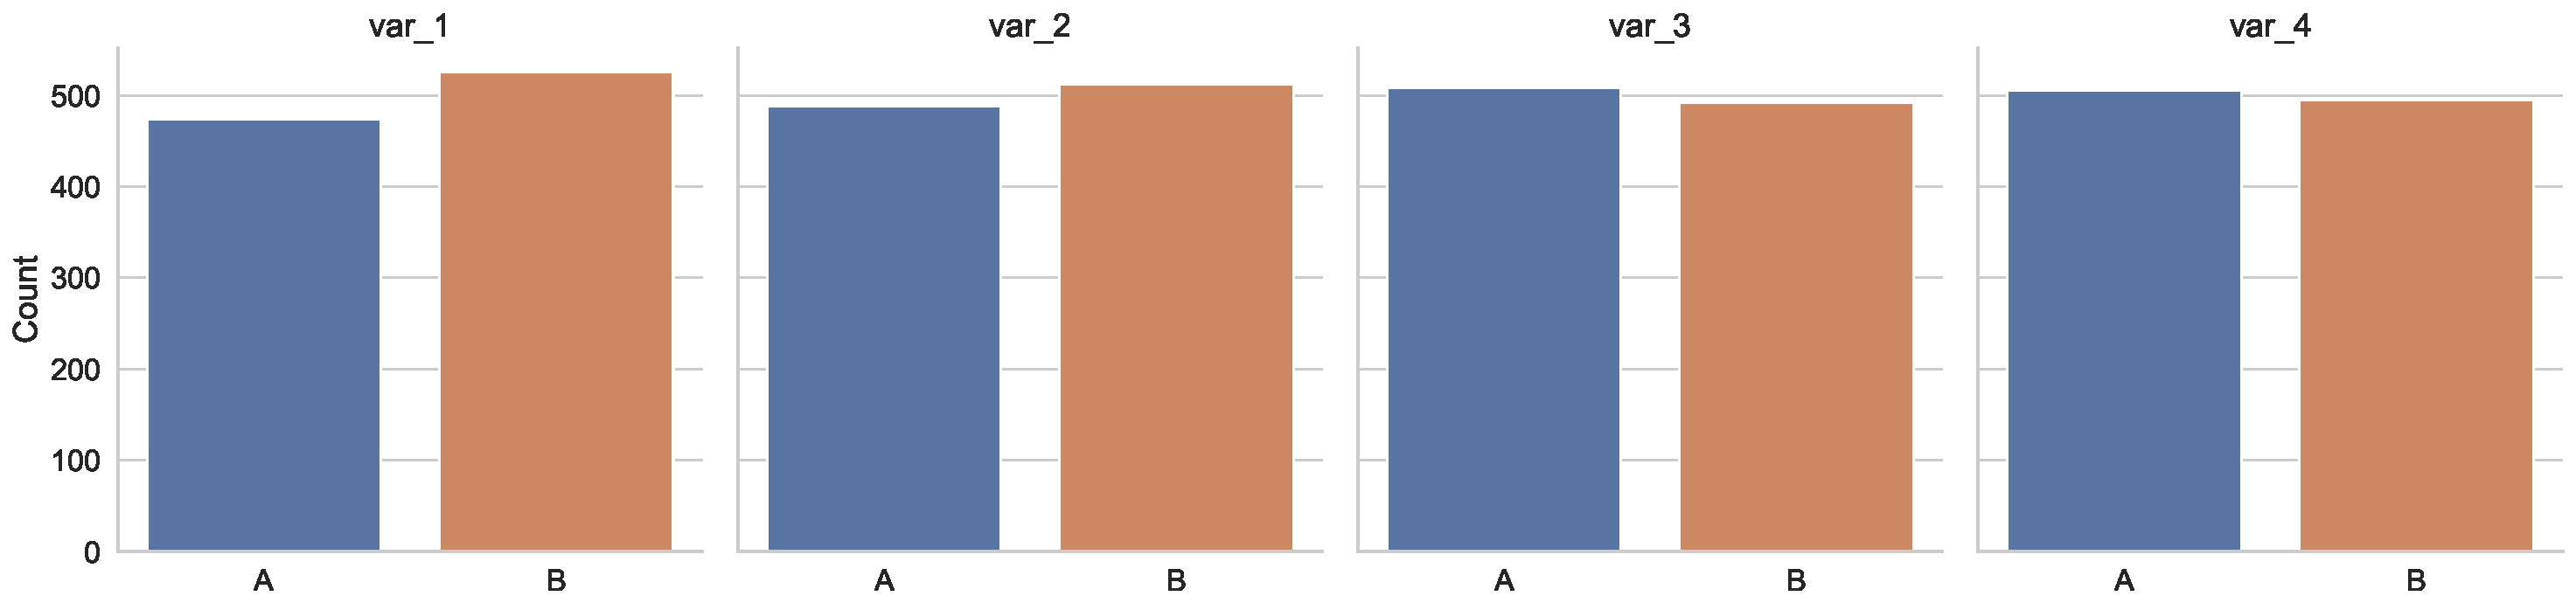
\includegraphics{../../simulation_data/categorical/graphs/graph_categorical.pdf}}
    \label{graph_categorical}
\end{figure}
}


\frame{\frametitle{Measuring utility in CTGAN}
\vspace{-5mm}
\begin{figure}
    \caption{}
    \resizebox{\textwidth}{!}{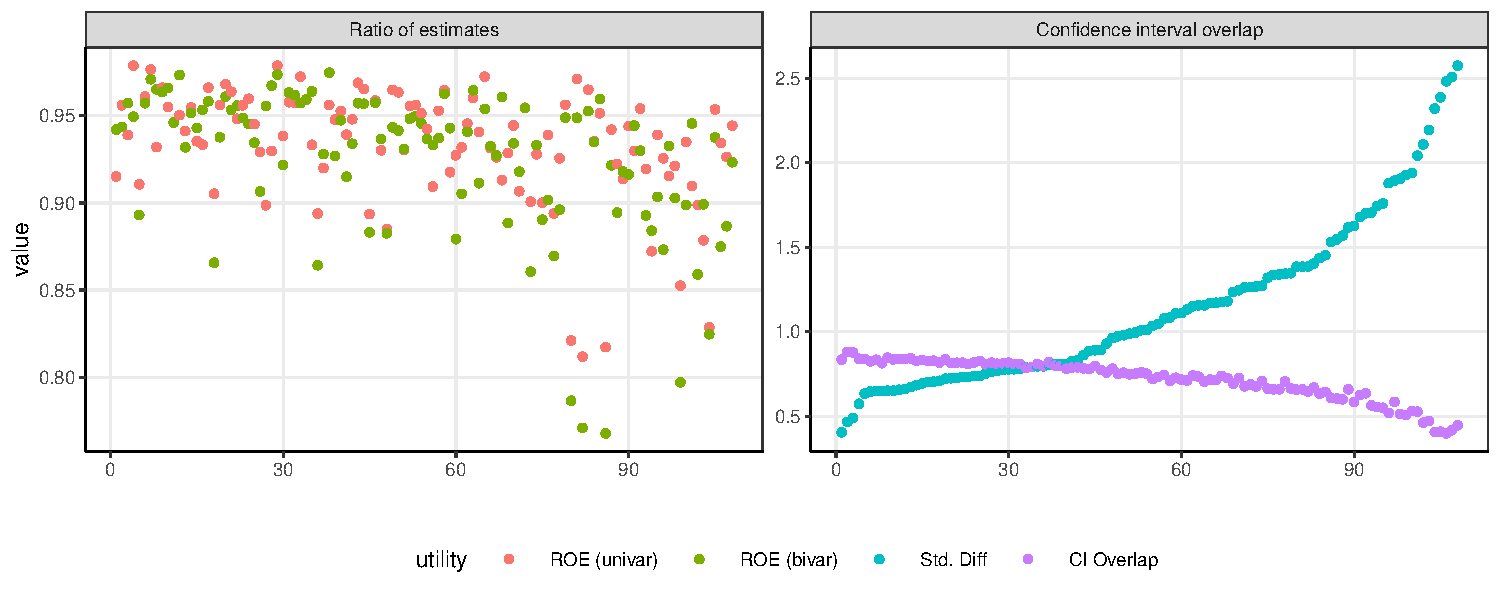
\includegraphics{../../simulation_data/categorical/graphs/ctgan/graph_compare_ctgan_utility.pdf}}
    \label{graph_compare_utility_sim_categorical_ctgan}
\end{figure}
}

\frame{\frametitle{Estimating ROE in CTGAN}
\vspace{-5mm}
\begin{figure}
    \caption{Parametric estimates from linear model}
    \resizebox{\textwidth}{!}{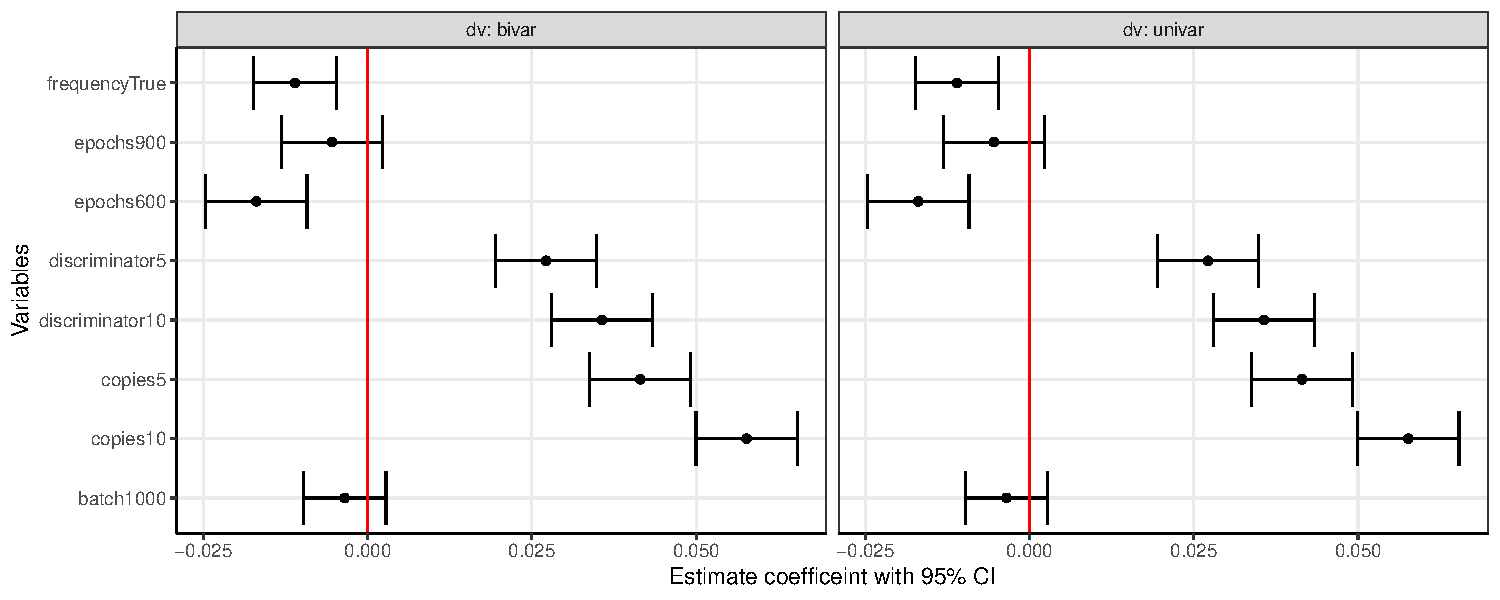
\includegraphics{../../simulation_data/categorical/graphs/ctgan/graph_ctgan_roe.pdf}}
    \label{graph_compare_utility_sim_categorical_ctgan_roe}
\end{figure}
}

\frame{\frametitle{Estimating ROE in CTGAN by copies ($m$)}
\vspace{-5mm}
\begin{figure}
    \caption{Parametric estimates from linear model}
    \resizebox{\textwidth}{!}{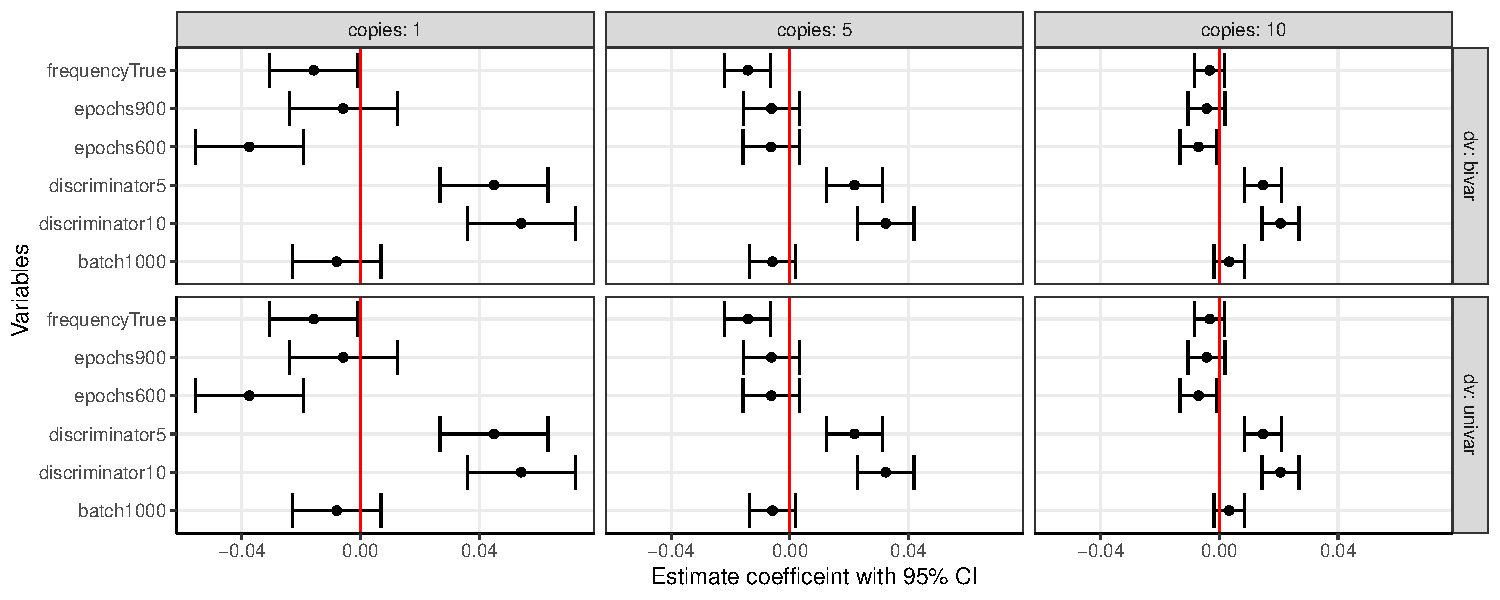
\includegraphics{../../simulation_data/categorical/graphs/ctgan/graph_ctgan_roe_copies.pdf}}
    \label{graph_compare_utility_sim_categorical_ctgan_roe_copies}
\end{figure}
}


\frame{\frametitle{Compare frequency counts between baseline and tuned}
\vspace{-5mm}
\begin{figure}
    \caption{}
    \resizebox{\textwidth}{!}{\includegraphics{../../simulation_data/categorical/graphs/graph_compare_frequency.pdf}}
    \label{graph_compare_frequency_categorical}
\end{figure}
}

\frame{\frametitle{Compare regression output between baseline and tuned}
\vspace{-5mm}
\begin{figure}
    \caption{}
    \resizebox{\textwidth}{!}{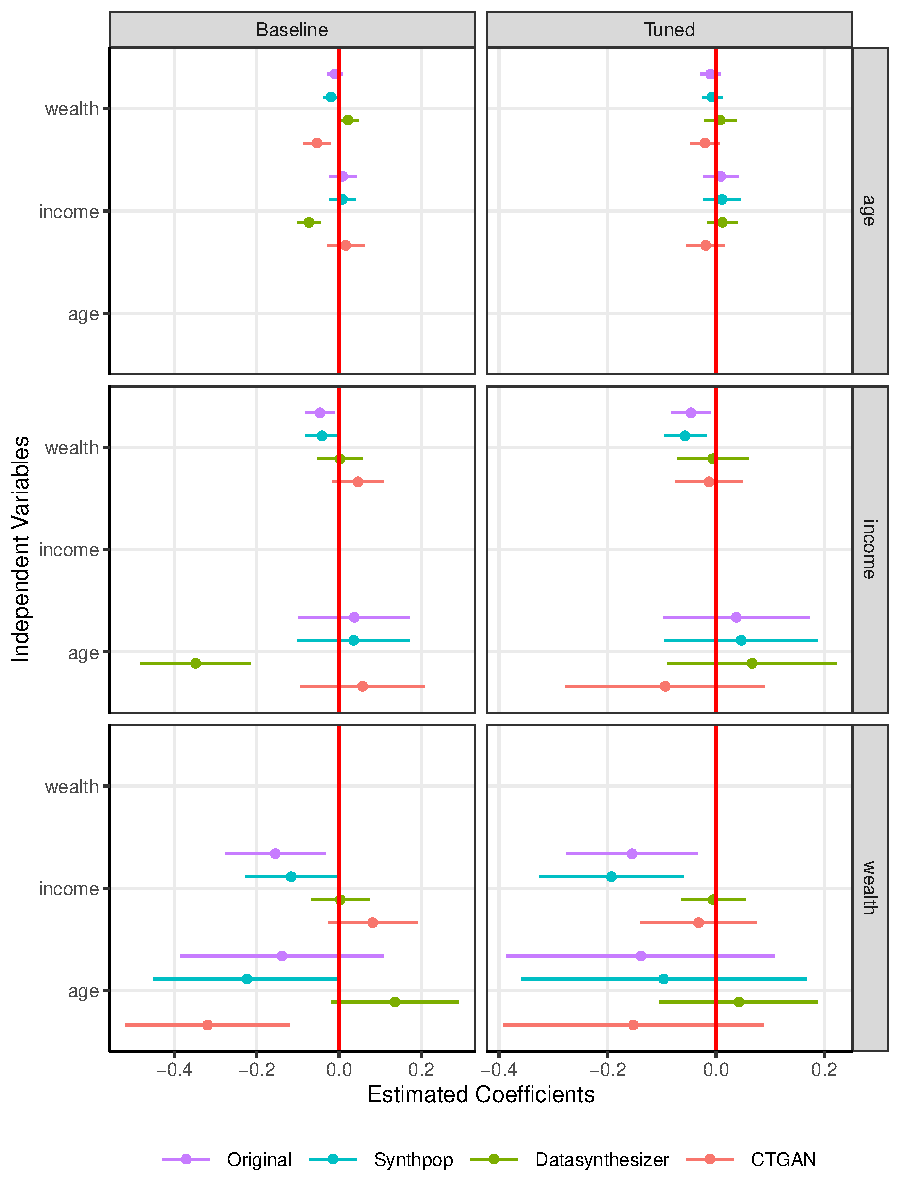
\includegraphics{../../simulation_data/categorical/graphs/graph_compare_cio_regressions.pdf}}
    \label{graph_compare_cio_regressions_categorical}
\end{figure}
}


\frame{\frametitle{Measuring utility for simulated categorical data}
\vspace{-5mm}
\begin{figure}
    \caption{}
    \resizebox{\textwidth}{!}{\includegraphics{../../simulation_data/categorical/graphs/graph_compare_utility.pdf}}
    \label{graph_compare_utility_sim_categorical}
\end{figure}
}


\subsection{Simulated continuous data}\label{sec_results_continuous}
\frame[c]{\frametitle{}
\centering
Section \ref{sec_results}: Results \\
Section \ref{sec_results}\ref{sec_results_continuous}: Simulated continuous data
}

\frame{\frametitle{Descriptive statistics - continuous variables}
\begin{table}[!h]
    \caption{}
    \centering
    \resizebox{\textwidth}{!}{\begin{tabular}{rlrrrrr}
\toprule
number & variable & min & max & mean & std & median \\
\midrule
1 & age & 16.00 & 94.00 & 55.65 & 22.56 & 57.00 \\
2 & income & 624.00 & 349355.00 & 35721.10 & 41455.86 & 22421.50 \\
3 & wealth & -19560.00 & 89975356.00 & 659520.71 & 3165853.95 & 127616.00 \\
\bottomrule
\end{tabular}
}
    \label{table_variables_continuous}
\end{table}
}

\frame{\frametitle{Measuring utility for simulated continuous data}
\vspace{-5mm}
\begin{figure}
    \caption{}
    \resizebox{\textwidth}{!}{\includegraphics{../../simulation_data/continuous/graphs/graph_compare_utility.pdf}}
    \label{graph_compare_utility_sim_continuous}
\end{figure}
}

\subsection{UK 1991}\label{sec_results_UK1991}
\frame[c]{\frametitle{}
\centering
Section \ref{sec_results}: Results \\
Section \ref{sec_results}\ref{sec_results_UK1991}: Individual Sample of Anonymised Records (SAR) for the British Census, subsetted on the region of West Midlands (UK 1991)
}

\frame{\frametitle{Descriptive statistics - UK 1991}
\vspace{-5mm}
\begin{figure}
    \caption{}
    \vspace{-5mm}
    \resizebox{\textwidth}{!}{\includegraphics{../../little_etal_2021/graphs/graph_descriptives.pdf}}
    \label{graph_descriptives}
\end{figure}
}

\frame{\frametitle{Measuring utility}
\vspace{-5mm}
\begin{figure}
    \caption{}
    \resizebox{\textwidth}{!}{\includegraphics{../../little_etal_2021/graphs/graph_compare_utility.pdf}}
    \label{graph_compare_utility}
\end{figure}
}

\frame{\frametitle{Frequency statistics}
\vspace{-5mm}
\begin{figure}
    \caption{}
    \vspace{-5mm}
    \resizebox{\textwidth}{!}{\includegraphics{../../little_etal_2021/graphs/graph_compare_frequency.pdf}}
    \label{graph_compare_frequency}
\end{figure}
}

\frame{\frametitle{Tuning Datasynthesizer}
\vspace{-5mm}
\begin{figure}
    \caption{}
    \vspace{-5mm}
    \resizebox{\textwidth}{!}{\includegraphics{../../little_etal_2021/graphs/graph_datasynthesizer_frequency_privacy.pdf}}
    \label{graph_datasynthesizer_frequency_privacy}
\end{figure}
}

\frame{\frametitle{Tuning Datasynthesizer}
\vspace{-5mm}
\begin{figure}
    \caption{}
    \vspace{-5mm}
    \resizebox{\textwidth}{!}{\includegraphics{../../little_etal_2021/graphs/graph_datasynthesizer_frequency_parents.pdf}}
    \label{graph_datasynthesizer_frequency_parents}
\end{figure}
}


\frame{\frametitle{Confidence interval overlap}
\vspace{-5mm}
\begin{figure}
    \caption{TENURE (Dependent variable)}
    \vspace{-5mm}
    \resizebox{\textwidth}{!}{\includegraphics{../../little_etal_2021/graphs/graph_compare_cio_tenure.pdf}}
    \label{graph_compare_cio_tenure}
\end{figure}
}

\frame{\frametitle{Confidence interval overlap}
\vspace{-5mm}
\begin{figure}
    \caption{MSTATUS (Dependent variable)}
    \vspace{-5mm}
    \resizebox{\textwidth}{!}{\includegraphics{../../little_etal_2021/graphs/graph_compare_cio_mstatus.pdf}}
    \label{graph_compare_cio_mstatus}
\end{figure}
}

\frame{\frametitle{Comparing duration to create 1 synthetic data set ($\times5$)}
\begin{table}[!h]
    \caption{UK 1991 data, 12 variables (1 continuous), and  $\approx$ 20.000 observations}
    \centering
    \input{../../little_etal_2021/tables/duration/table_duration.tex}
    % \resizebox{\textwidth}{!}{\input{../../little_etal_2021/tables/duration/table_duration.tex}}
    \label{table_dution_UK1991}
\end{table}
}

\subsection{SD 2011}\label{sec_results_SD2011}
\frame[c]{\frametitle{}
\centering
Section \ref{sec_results}: Results \\
Section \ref{sec_results}\ref{sec_results_SD2011}: Social Diagnosis 2011 (SD2011)
}

\frame{\frametitle{Descriptive statistics - SD2011}
\vspace{-5mm}
\begin{figure}
    \caption{}
    \resizebox{\textwidth}{!}{\includegraphics{../../SD2011/graphs/graph_descriptives.pdf}}
    \label{graph_descriptives}
\end{figure}
}

\frame{\frametitle{Measuring utility}
\vspace{-5mm}
\begin{figure}
    \caption{}
    \resizebox{\textwidth}{!}{\includegraphics{../../SD2011/graphs/graph_compare_utility.pdf}}
    \label{graph_compare_utility}
\end{figure}
}

\frame{\frametitle{Confidence interval overlap}
\vspace{-5mm}
\begin{figure}
    \caption{}
    \resizebox{\textwidth}{!}{\includegraphics{../../SD2011/graphs/graph_compare_cio.pdf}}
    \label{graph_compare_cio}
\end{figure}
}

\frame{\frametitle{Comparing duration to create 1 synthetic data set ($\times5$)}
\begin{table}[!h]
    \caption{SD 2011, 4 variables (2 continuous), and $\approx$ 5.000 observations}
    \centering
    \input{../../SD2011/tables/duration/table_duration.tex}
    % \resizebox{\textwidth}{!}{\input{../../little_etal_2021/tables/duration/table_duration.tex}}
    \label{table_dution_SD2011}
\end{table}

$^*$ Synthpop $<$ 1 second
}

\section{Conclusion}\label{sec_conclusion}
\frame[c]{\frametitle{}
\centering
Section \ref{sec_conclusion}: Conclusion
}

\frame{\frametitle{Summary}
\vskip -3mm
\begin{itemize}
    \footnotesize
    \item Main message: Synthpop is the `winner'
    \begin{itemize}
        \footnotesize
        \item Highest utility
        \item Fastest
        \item Little tuning required 
    \end{itemize}
    \item Datasynthesizer
    \begin{itemize}
        \footnotesize
        \item Requires tuning
        \begin{itemize}
             \item Baseline assigns equal distribution to values within any variable
             \item $k$ parents that are too high returns baseline (without warning)
         \end{itemize} 
    \end{itemize}
    \item CTGAN
    \begin{itemize}
        \footnotesize
        \item Slowest
        \item Worst performing 
    \end{itemize}
\end{itemize}
}

\frame{\frametitle{Next steps}
\begin{itemize}
    \footnotesize
    \item Simulation data
    \begin{itemize}
        \footnotesize
        \item Mixed data (categorical and continuous)
        \item Correlated variables
        \item Missing values 
    \end{itemize}
    \item Different measures of utility
    \item Different packages for creating synthetic data
    \begin{itemize}
        \footnotesize
        \item Simcity
        \item 
    \end{itemize}
    \item Privacy
\end{itemize}
}

\frame{\frametitle{Questions}
\begin{itemize}
    \footnotesize
    \item Whats my story?
    \item Is there different data that would tell a different story (i.e. relational databases)
    \item When do GANs perform well?  (i.e. not socio-economic data)
\end{itemize}
}


\frame[c]{\frametitle{}
\centering
Thank you
}


\end{spacing}

\end{document}

